\label{chapter:case-studies}
%
We have formalized variational \ac{smt} and \ac{sat} solving. However, we have
yet to investigate the performance of our methods. Recall from
\autoref{chapter:introduction} that a motivating reasons for a variational
solver was that if we only compute shared terms once, then we should observe a
speedup in runtime performance when solving sets of related \ac{sat} problems
because information is reused. In this chapter, we investigate and verify these
claims.

Assessing the performance of \ac{sat} and \ac{smt} solvers is notoriously
difficult~\cite{Gent94thesat} because it depends on the input problem to the
\ac{sat} or \ac{smt} solver. The issue is related to the computational hardness
of the input. Hardness, in this domain is estimated by the ratio of clauses in
the \ac{sat} or \ac{smt} problem to the number of variables. Conceptually, if
there are many clauses and not many variables then the problem is
over-constrained and it is easy to decide \rn{unsat}, however if there are few
clauses but many variables then the problem is under-constrained and it is easy
to decide \rn{sat}. Thus, hard problems rest in a \emph{phase transition} zone
where the ratio of clauses to variables is neither over-constrained nor
\todo{cite}under-constrained.

To investigate the performance of our methods, we construct a prototype
variational solver, \vsat{} in the Haskell programming
language~\cite{Hudak:1992:RPL:130697.130699} and quantitatively compare it to
incremental and non-incremental \ac{sat} solving. Assessing the prototype in
realistic conditions is difficult as there does not exist a corpus of accepted
representative variational \ac{sat} problems. Thus, to test the prototype in as
realistic conditions as possible we utilize real-world data from a previous
study by~\citet{NMS+:GPCE18} from the \ac{spl} community.

Before we describe the datasets and resulting variational \ac{sat} problems we
first introduce some terminology from the \ac{spl} community. A software
product-line is an instance of variational software; \todo{get a source here}or
more formally it is a set of software-intensive systems that share a common,
managed set of features satisfying the specific needs of a particular market
segment or mission and that are developed from a common set of core assets in a
prescribed way.

A good example of a software product-line is the Linux kernel~\cite{linux}. The
Linux kernel is a set of core assets which devise an operating system, but the
assets are parameterized by \emph{features} which, in this case, are the Boolean
conditions of conditional-compilation statements such as \cpp{ifdef}s. To select
the particular kind of kernel to build, the Linux kernel uses the
\texttt{KConfig}~\cite{kconfig} tool to enable or disable features and thus
specify the exact kernel to build. The set of features and their dependencies
which determine the product, or in this case determine the kernel that is built
is call a \emph{feature model}\cite{KCHNP90}.

It is common to express feature models as a \ac{sat} formula where variables are
features, and dependencies are expressed using logical connectives. Thus,
reasoning about feature models with a \ac{sat} solver is an active sub-field in
\acl{spl}~\cite{BSRC10,GBT+19,BSTRC06,TAK+:SE15}. For example, a \emph{void
  analysis} uses a \ac{sat} solver to determine that a product is possible, and
a \emph{core analysis} manipulates the feature model to check that a given
feature must be \tru{} (or enabled in the \ac{spl} terminology) for every viable
product. Conceptually in this domain, if a \rn{sat} is returned from the solver
then the resulting model is an assignment of features which specifies a viable
product. If an \rn{unsat} is returned than no viable product exists given the
constraints on the feature model for the software product-line. Further analysis
on the product line are

\section{Experimental Methodology}
~\label{section:case-studies:experimental-methodology}
%
For the remainder of the chapter, we must distinguish between concepts in the
application domain, such as a void or core analysis, and concepts in the solver
domain, such as a query or choice. In general, we focus on the solver domain as
it is our primary concern.

\nieke{} provides two datasets\footnote{see
  \url{https://gitlab.com/evolutionexplanation/evolutionexplanation}},
\textit{automotive02} and \textit{financialServices1} which encode the evolution
histories of two feature models as propositional formulas. We refer to these as
the \auto{} dataset, and \fin{} dataset for the remainder of this chapter. Since
these datasets encode evolution histories, variants in our analysis correspond
to snapshots of feature models over time, and a plain model of a variant
corresponds to a void analysis over that feature model. For example, a variant
of the \auto{} dataset is a \pl{} formula which encodes a feature model at time
0, and another variant encodes \emph{the same} feature model at time 2, where $0
< 2$. Recall the possible existence of extra variants from
\autoref{section:vpl:example}, since extra variants may exist given a \ac{vpl}
encoding of the datasets we use the phrase \textit{version variant} to refer to
variants that are snapshots of a feature model in the application domain. For
example, the variant which corresponds to a feature model at time 0 is a version
variant, but the variant which corresponds to a feature model at time 0
\emph{and} and time 2 are non-version variants.

We assess the performance characteristics \vsat{} by attempting to answer the
following research questions.
%
\begin{enumerate}%[align=left]
\item[\resQ{1}] How does variational solving scale as variation increases?
\item[\resQ{2}] What is the impact of base solvers on performance?
\item[\resQ{3}] What is the impact of sharing on performance?
\item[\resQ{4}] What is the cost of solving a plain formula on \vsat{}?
\end{enumerate}

To investigate \resQ{1} and \resQ{2}, we consider all variants of the \ac{vpl}
formulas constructed for each dataset, rather than just the version variants
that are of interest in the application domain. This allows us to better
evaluate how \vsat{} scales to accommodate variability.
%
For \resQ{3}, we hypothesize that \vsat{} will show observable speedups as
sharing increases, which would validate our method of deriving a variational
core. To investigate this, we restrict the analysis to consecutive version
variants (i.e., consecutive monthly snapshots of a feature model), and observe
performance as sharing is left uncontrolled.
%
Finally, \resQ{4} provides insight on the overhead incurred by variational
solving, which we investigate by inputting each version variant as a
propositional logic formula rather than a single variational formula for each
solver used in \resQ{2} and \resQ{1}.

\subsection{Data Description and Encoding}%
\label{section:exper-meth:description}
%
\nieke{}'s formulas collapse sets of \pl{} formulas to a single formula using
implications on an \ac{smt} variable that represents a moment in time. A
two-pass process was used to translate \nieke{}'s formulas into \ac{vpl}---one
pass to parse to an internal representation and another to detect and convert
\nieke{}'s temporal ranges to choices, nesting the implied clauses into the true
alternative.

The two datasets differ in important ways. The \auto{} dataset encodes four
monthly snapshots while the \fin{} dataset encodes ten. Hence, the \auto{}'s
query formula represents 16 variants, while the \fin{} query formula represents
1,024 variants. For \resQ{3} and \resQ{4}, we construct several \vc{}'s to
restrict the analysis to version variants. The \vc{}s range from ones that
enable only one version variant (for \resQ{4}): $\kf{vc_{\kf{auto\_V_{1}}}} =
(V_{1} \wedge \neg V_{2} \wedge \neg V_{3} \wedge \neg V_{4})$ to \vc{}s that
enable only consecutive version variants (for \resQ{3}):
$\kf{vc_{\kf{auto\_V12}}} = V_{1} \veebar V_{2}$.

For \resQ{4} we decouple performance from the number of variants by performing
an initial pass over the query formula to replace choices representing
non-consecutive versions variants (\eg{} a variational formula which represents
$V_{1}$ and $V_{2}$ but not $V_{1}$ and $V_{3}$) with their false alternatives
(which contain the value \tru{}). Then we construct a \vc{} to forbid
non-version variants. As an example, the \auto{} dataset, yields three data
points by this process, the change from versions $V_{1}$ to $V_{2}$, $V_{2}$ to
$V_{3}$, and $V_{3}$ to $V_{4}$. All results presented for \resQ{3} were
  calculated using the z3~{\citep{10.1007/978-3-540-78800-3_24}} \ac{sat}
  solver.

\paragraph{Measuring Performance}%
\label{section:exper-meth:perf}
%
To answer our research questions, we construct four different solving
algorithms using our prototype tool. We use the notation
\iToj{<formula>}{<solver>} to describe, for each algorithm, whether the query
formulas and solver are plain ($p$) or variational ($v$), respectively.
%
The algorithms are: the baseline, \pTop{}, which runs plain formulas on a plain
solver; the variational case, \vTov{}, which runs a variational formula on the
variational solver; the overhead case, \pTov{}, which runs plain formulas on the
variational solver; and the typical case, \vTop{}, which runs the variational
formula, variant by variant, on a plain solver. Inputs for each algorithm are
constructed by configuring the query formula, thus ensuring that the same
variation context is used across algorithms.

We construct the \pTop{} algorithm by configuring the query formula to its
variants \textit{before} benchmarking begins. These formulas are then sent to
the base solver one-by-one, with the solver begin shut down and initialized
between runs, thus preventing the solver form maintaining any learned
information.
%
The \pTov{} case corresponds to \resQ{4} and elucidates the potential overhead
of solving a plain query on a variational solver. We perform the same
pre-processing as the \pTop{} case but send each plain formula to \vsat{}
instead. This provides insight into the cost incurred by the reduction engine.
%
For \vTop{}, we configure the query formula to retrieve variants \textit{during}
benchmarking. Each formula is sent to the base solver \textit{with} the solver
maintaining information between queries. This gives insight into the overhead
incurred by configuring a variational formula, and the benefits of the internal
caching in the base solver. Notable, this case keeps the base solver running,
performing each call in incremental mode, thus this case corresponds to the
typical use of an incremental solver in applications that utilize incremental
\ac{sat} solvers.

We construct a variational model for all algorithms since it is unclear how to
combine plain models, and since the storage of plain models is an orthogonal
concern to performance, we sought to keep convolved variables constant.

Unless specified, all results are a bootstrapped statistical average
representing numerous raw measurements.\footnote{Using v0.2.5 of the
  gauge~\citep{gauge} library and v8.6 of the sbv~\citep{sbv} library with
    solver seeds set to \texttt{1729}. All data was collected on a desktop
    running NixOS 20.09, with an AMD Ryzen 7 2700X CPU @ 4.0GHz, 32GB RAM.\@We
    used stack lts-15.7 (GHC 8.8.3) and tested with RTS options ``-qg'' which
    enables parallel garbage collection in the Haskell runtime.}
%
  For \resQ{2} we repeat \resQ{1} with four different base solvers:
  z3~\cite{10.1007/978-3-540-78800-3_24},
  cvc4~\citep{10.1007/978-3-642-22110-1_14}, yices~\citep{Dutertre:cav2014} and
  boolector~\citep{DBLP:conf/tacas/BrummayerB09}, each of which called through
  the widely used Haskell library~\citep{sbv}. To assess \resQ{2} we perform a
  Kruskall-Wallis test~\citep{nist} followed by a pairwise Wilcox
  test~\citep{WilcoxonPairwise} with Holm-Bonferroni p-value
  correction~\citep{10.2307/4615733} in the R programming language~\citep{RLang}
  v4.0.3 and assume a 5\% significance level.
%
For \resQ{3}, we similarly normalize the data to the baseline (\vTop{}), fit a
linear model, and statistically assess differences by repeating the
aforementioned statistical tests. For \resQ{4}, we retrieve the raw measurements
from the bootstrapped average and assess statistical differences identically to
\resQ{3} but do not fit any models to the data. Furthermore, the variational
input is nuanced for \resQ{4} as each data point is on a variant, which is
necessarily plain. Thus, \resQ{4} is a special case; for \resQ{4} \vTov{} inputs
the variational formula but utilizes a variant context to restrict the solver to
the version variant. \vTop{} performs configuration to configure for the version
variant and then runs the variant on a base solver during benchmarking. All
results, including variational models and statistical analysis scripts, are
available online.\footnote{\github{}}

%%% Local Variables:
%%% mode: latex
%%% TeX-master: "../../thesis"
%%% End:
%
\section{Results and Discussion}
\label{section:case-studies:results-and-discussion}
%
\begin{figure}
  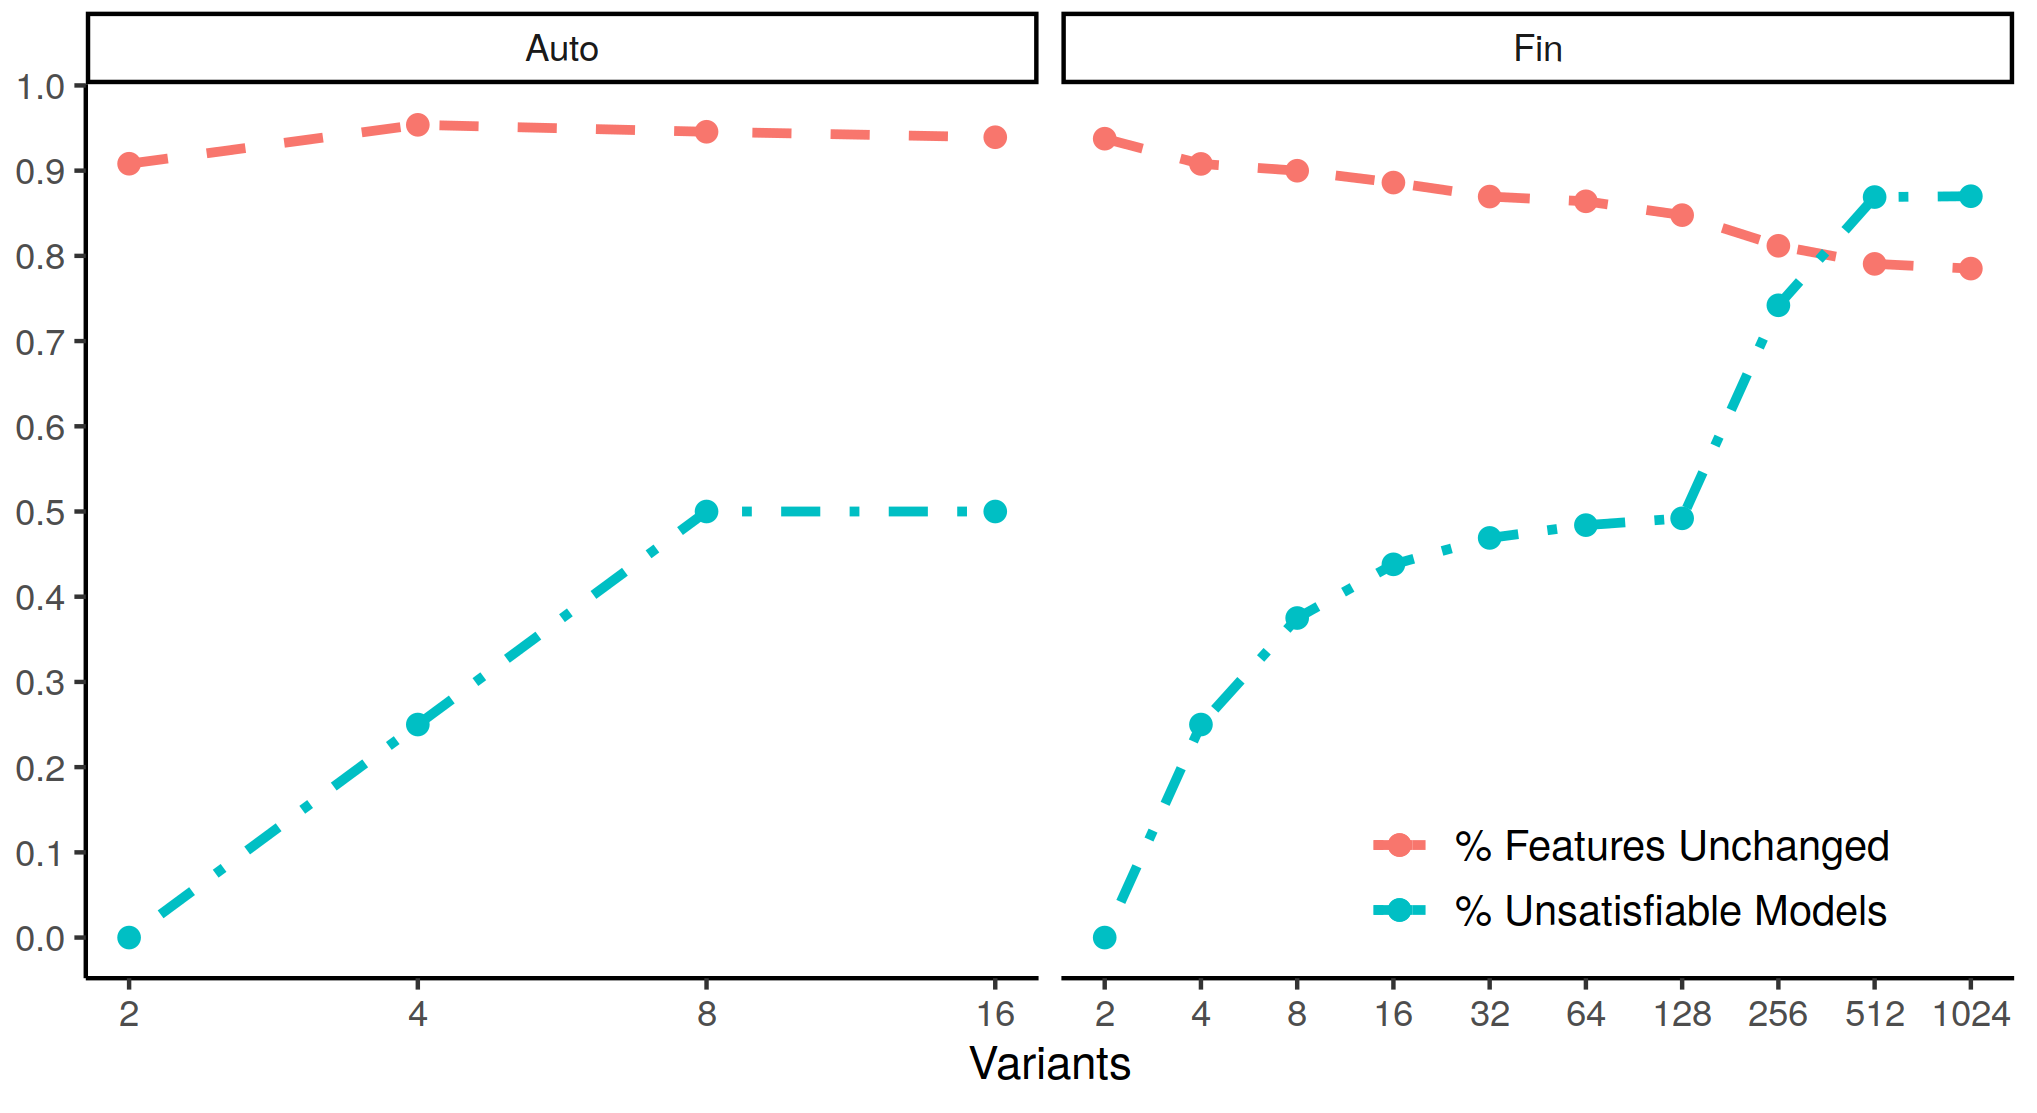
\includegraphics[width=0.95\textwidth]{Plots/VModel}
  \caption{Ratio of models found to be unsatisfiable.}%
  \label{res:vmodels}
\end{figure}
%
The datasets yielded dissimilar query formulas: the \auto{} query formula
consisted of 4,212 choice terms (not including terms in a choice's
alternatives), and 26,808 plain terms. In contrast, \fin{} had 3,809 choice
terms, and 1,441 plain terms. Thus \fin{} had larger changes between product
line versions. \autoref{res:vmodels} shows the ratio of unsatisfiable models to
total plain models, and the ratio of constant features for each product line
version (represented by variant count). For both datasets the number of
satisfiable models decreased as new versions were considered, and the majority
of features in each model never flipped from their initialized value \fls{} to
\tru{}. Thus, the variational model is likely a compressed version of the set
of plain models. Compression metrics were not calculated as this is an
orthogonal concern to the performance of variational satisfiability solving.

Variational models permit product analyses without a \ac{sat} solver.
\autoref{res:vmodels} shows such a purely syntactic analysis: counting
disjuncted clauses in the variational model as a representation of satisfiable
plain models. We believe post-hoc analyses such as this may be useful to feature
modelers as they direct attention to impactful versions of the feature model.
For example, the change from $V_{7}$ to $V_{8}$ (128 to 256 Variants) of \fin{}
clearly constrained the feature model as the number of unsatisfiable models
increased from 50\% to 80\%.

The experiment required 7 days, 6 hours and 21 minutes to complete. Due to the
amount of time required to generate the data, we limited the number of raw
measurements to 3. Thus, each data point presented in our results is a
bootstrapped average of 3 raw measurements.

\subsection{RQ1: Performance of Variational Solving as Variation Scales}

\begin{figure}
  \centering
  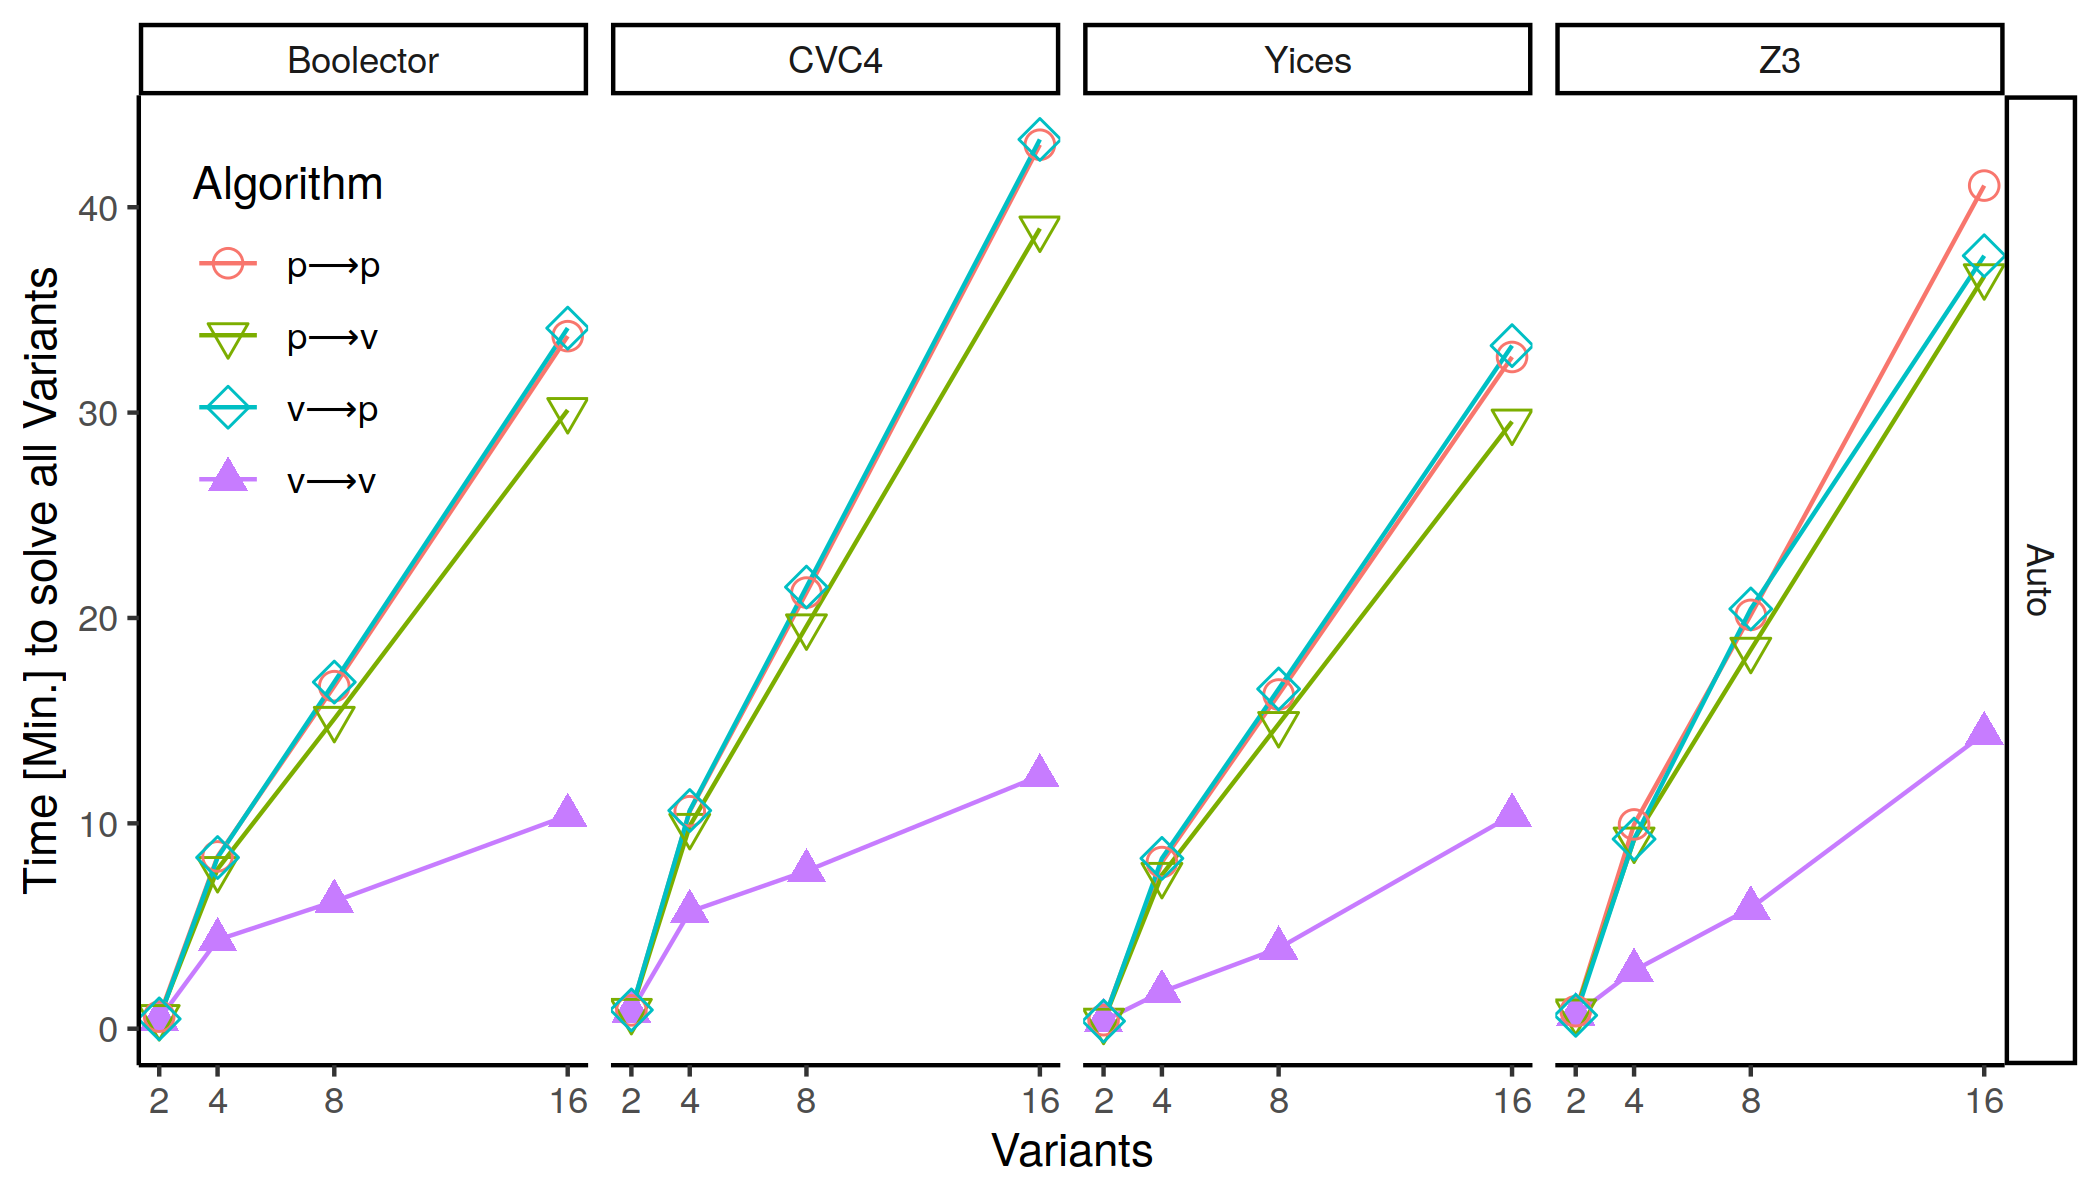
\includegraphics[width=0.95\textwidth]{Plots/RQ1_Auto}
  \caption{(Auto) RQ1: performance as variants increase per base solver. \vTov{}
    shows a speedup of 2.8--3.5x for the \auto{} dataset depending on base
    solver.}%
  \label{res:rq1:auto}
\end{figure}
%
\begin{figure}[h]
  \centering
  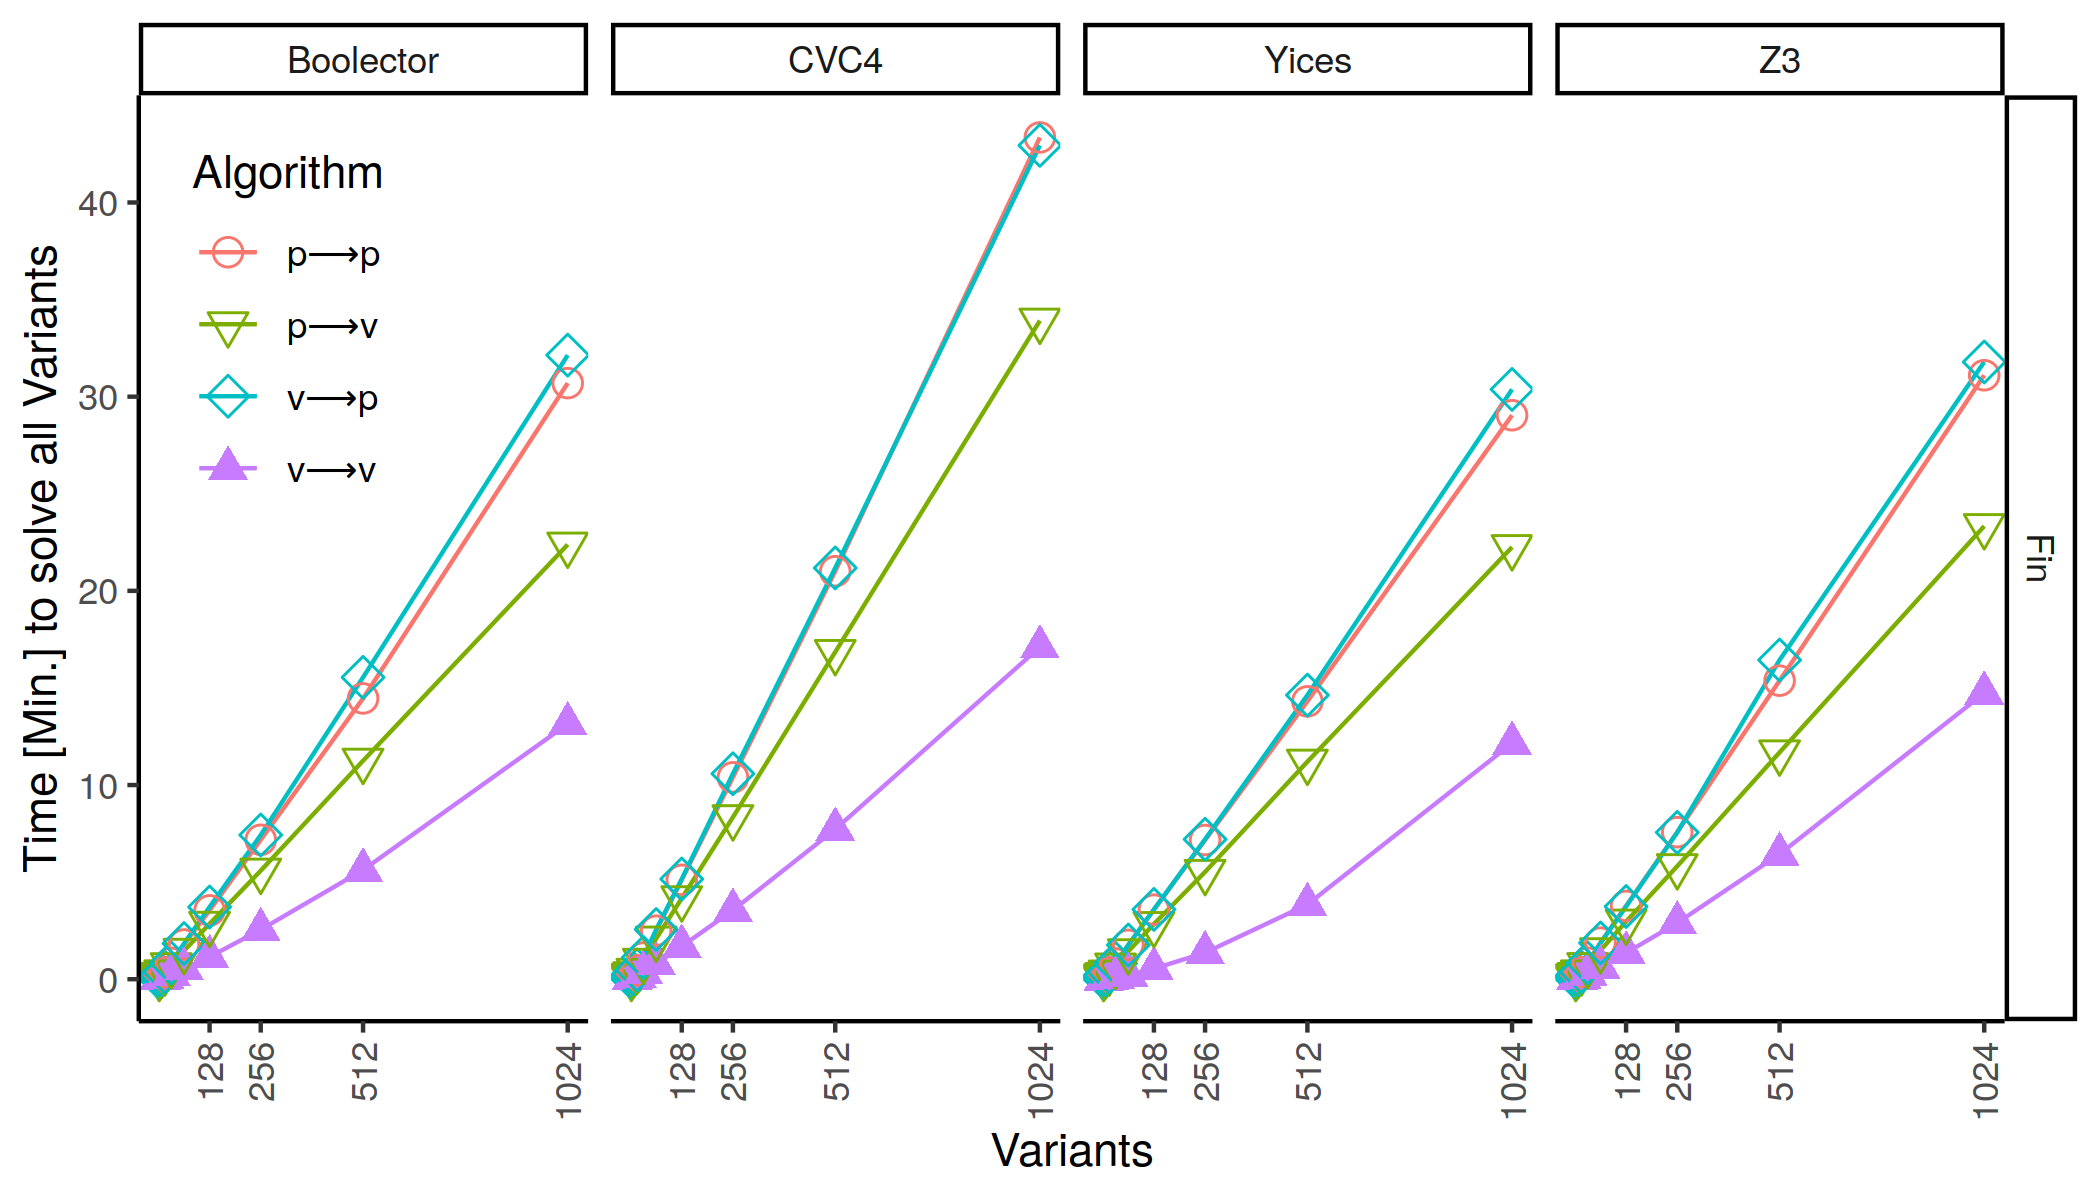
\includegraphics[width=0.95\textwidth]{Plots/RQ1_Fin}
  \caption{(Financial) RQ1: performance as variants increase per base solver. \vTov{}
    shows a speedup of 2.4--3.2x for the \fin{} dataset depending on the base
    solver. Overlapping x-axis labels elided.}%
  \label{res:rq1:fin}
\end{figure}

\begin{table}
  \begin{subtable}[t]{0.45\textwidth}
    \centering
    \begin{tabular}{c || c | c | c | c}
      DataSet    & Boolector & CVC4 & Yices & Z3 \\
      \hline
      \auto{}    & 3.29      & 3.51 & 3.20  & 2.62 \\
      \fin{}     & 2.44      & 2.51 & 2.50  & 2.16 \\
    \end{tabular}
    \caption{Speedup by solver for the maximum variant case; 16 for \auto{},
      1024 for \fin{}.}%
    \label{tab:rq1:speedup}
  \end{subtable}
  \hfill
  \begin{subtable}[t]{0.45\textwidth}
    \centering
    \begin{tabular}{ c | c | c | c}
      Boolector & CVC4 & Yices & Z3 \\
      \hline
       623.0    & 738.6 & 623.7 & 862.0 \\
       788.8     & 1026.6 & 729.2  & 884.2 \\
    \end{tabular}
    \caption{Time [s] to solve with \vTov{} by solver.}%
    \label{tab:rq1:comparison}
  \end{subtable}
  \caption{Time to solve and speedup of most variational case by solver.}%
  \label{tab:rq1}
\end{table}

The \vsat{} tool outperforms other algorithms as the count of variants to solve
increases for every base solver. \autoref{res:rq1:auto} shows the time to solve
the query formula as variants increase from 2 to 16 for the \auto{} dataset for
each solver. Similarly \autoref{res:rq1:fin} shows time to solve by base solver
for the \fin{} dataset.

For the \auto{} dataset, variational solving is faster with an average speedup
of 2.60x. For the most variational case (16 variants) the greatest speedup was
found to be 3.5x with cvc4. The \fin{} dataset shows an average speedup of
4.70x~\footnote{Due to extreme outliers (10x--15.1x speedup) from yices when
  solving 2--32 variants.}. For the most variational case (1024 variants), cvc4
also showed the greatest speedup at 2.51x. We find that \vTov{} is statistically
different from every other algorithm with p-values of $2.77\times 10^{-4}$
(\vTop{}), $1.06\times 10^{-2}$ (\pTop{}), and $1.92\times 10^{-2}$ (\pTov{})
for \auto{} and $1.62\times 10^{-5}$ (\vTop{}), $1.92\times 10^{-5}$ (\pTop{}),
and $1.70\times 10^{-4}$ (\pTov{}) for \fin{}.

\vsat{} outperforms the other algorithms because the variational core caches
plain terms, thereby preventing the re-evaluation of these terms for each
variant. By this data, we observed a constant factor speedup. Thus, variational
solving still grows linearly in the number of variants being solved.


\subsection{RQ2: Performance Impact of Base Solver}
%
From \resQ{1} we determined that \vTov{} is faster than the baseline algorithms
and that the difference is statistically significant. We observe from
\autoref{res:rq1:auto} and \autoref{res:rq1:fin} that the \vTov{} algorithm is
robust across every tested base solver and \vTov{} produced reasonable results
with each base solver.
%
We summarize our results in \autoref{tab:rq1}. Notable yices was consistently
the most performent base solver for all algorithms and all test cases. For
\vTov{} yices demonstrates not only a high degree of speedup but also a
reduction of 238.3 seconds, and 132.8 seconds, in run time from z3 for the
most variational case of \auto{} and \fin{}. Thus, yices is an attractive
target for the base solver of future prototype variational \ac{sat} solvers.

Cvc4 is also noteworthy; cvc4 benefited the most from \vTov{} for both
datasets with a speedup 3.51x (\auto{}) and 2.51 (\fin{}). The cvc4 case is
interesting as it implies that a base solver which shows poor performance with
in the typical use case (\vTop{}; \ac{sat} calls occur in an incremental
constext, and solver is kept alive) may greatly benefit from the variational
solving algorithm we've presented. Although the exact reasons behind this
behavior will be particular to the base solver, these results imply that our
use case (\ie{}, heavily exercising the incremental code paths) is peculiar
and thus selecting a solver based on only its typical performance may not be
representative of its performance in this use case.

\subsection{RQ3: Performance Impact of Plain Terms}
We hypothesize that the ratio of plain terms to total terms should increase the
variational solver's performance. Specifically, we hypothesize that as sharing
grows, the query formula's variational core is further reduced. We observe this
behavior using the z3 data in \autoref{res:speedup}. Both \vTov{} and \pTop{}
showed a statistically significant fit to a linear model. Furthermore, only
\vTov{} was found to be statistically different from \pTop{} and \pTov{} with
p-values of $6.95\times 10^{-3}$ and $4.44\times 10^{-6}$ thus confirming that
sharing positively correlates to speedups for variational solving in these
datasets.

This result is evidence that a dataset's sharing ratio is an important factor in
the performance of a variational \ac{sat} solver, as we hypothesized. When the
sharing ratio is high, the reduction engine produces a smaller variational core.
With a smaller variational core, more reuse of plain terms occurs and thus
computational time is saved in the base solver. Hence, an avenue of future work
is to leverage the laws of the variational logic to automatically refactor input
formulas to increase sharing. The consequences of this observation will be
particular to the application domain. For software product lines this means that
any method to increase sharing between product line versions or the
representative \ac{sat} problems is desirable; this may be smaller changes with
respect to the entire feature model, more frequent snapshots of the feature
model, or syntactic manipulations to mitigate the occurrence of new features.

\begin{figure}
  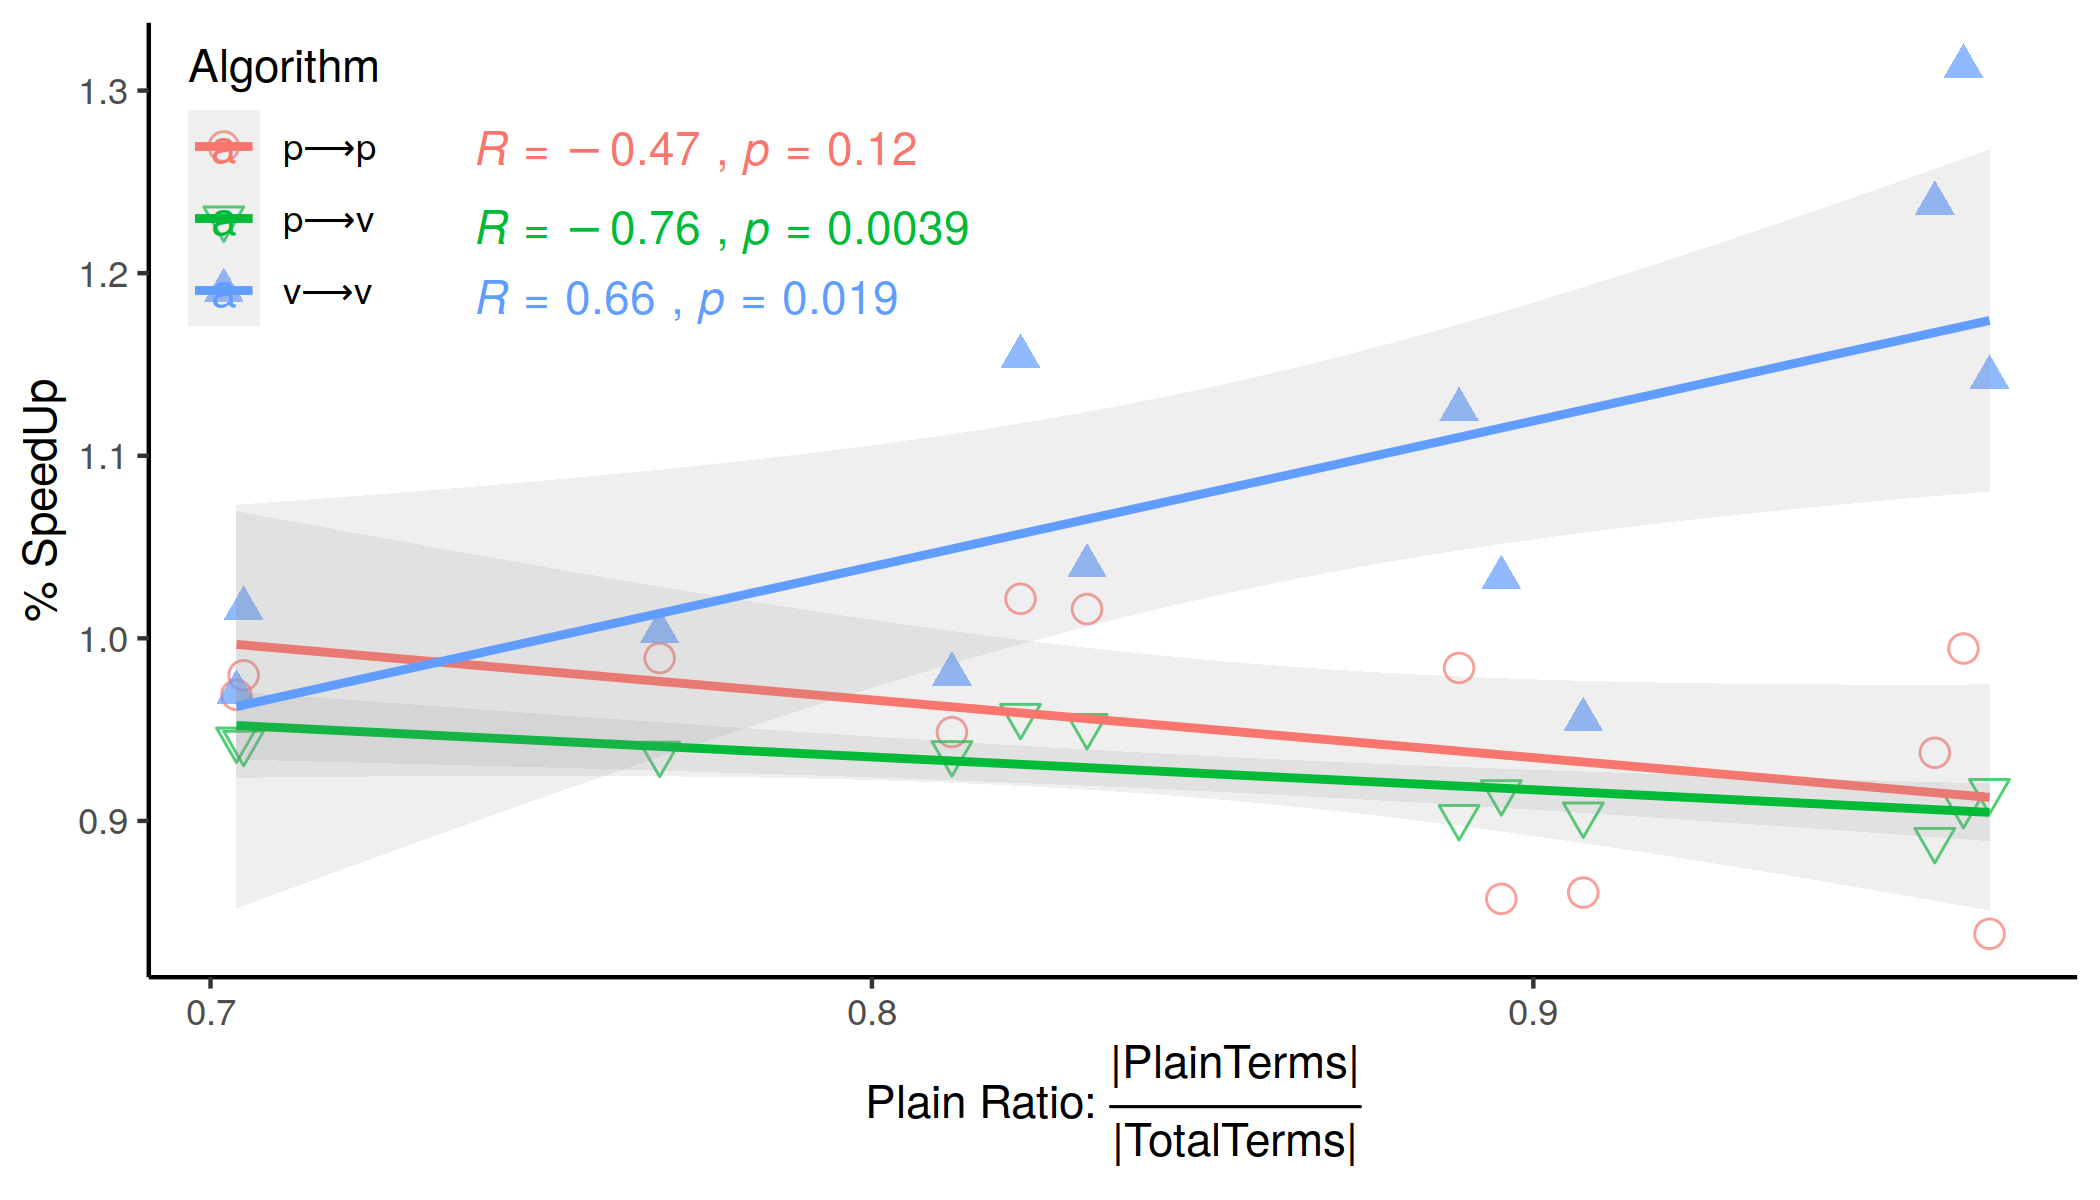
\includegraphics[width=0.95\textwidth]{Plots/RQ3}
  \caption{RQ3: performance as a function of plain ratio. We observe that
    sharing positively correlates to speedup only for \vTov{}, where $\texttt{\%
      SpeedUp} = \frac{{\text{Algorithm}}}{{\text{\vTop{}}}}$.}%
  \label{res:speedup}
\end{figure}

\subsection{RQ4: Overhead of a Plain Query on \vsat{}}
%
\begin{figure}
  \begin{subfigure}[t]{\textwidth}
    \centering
    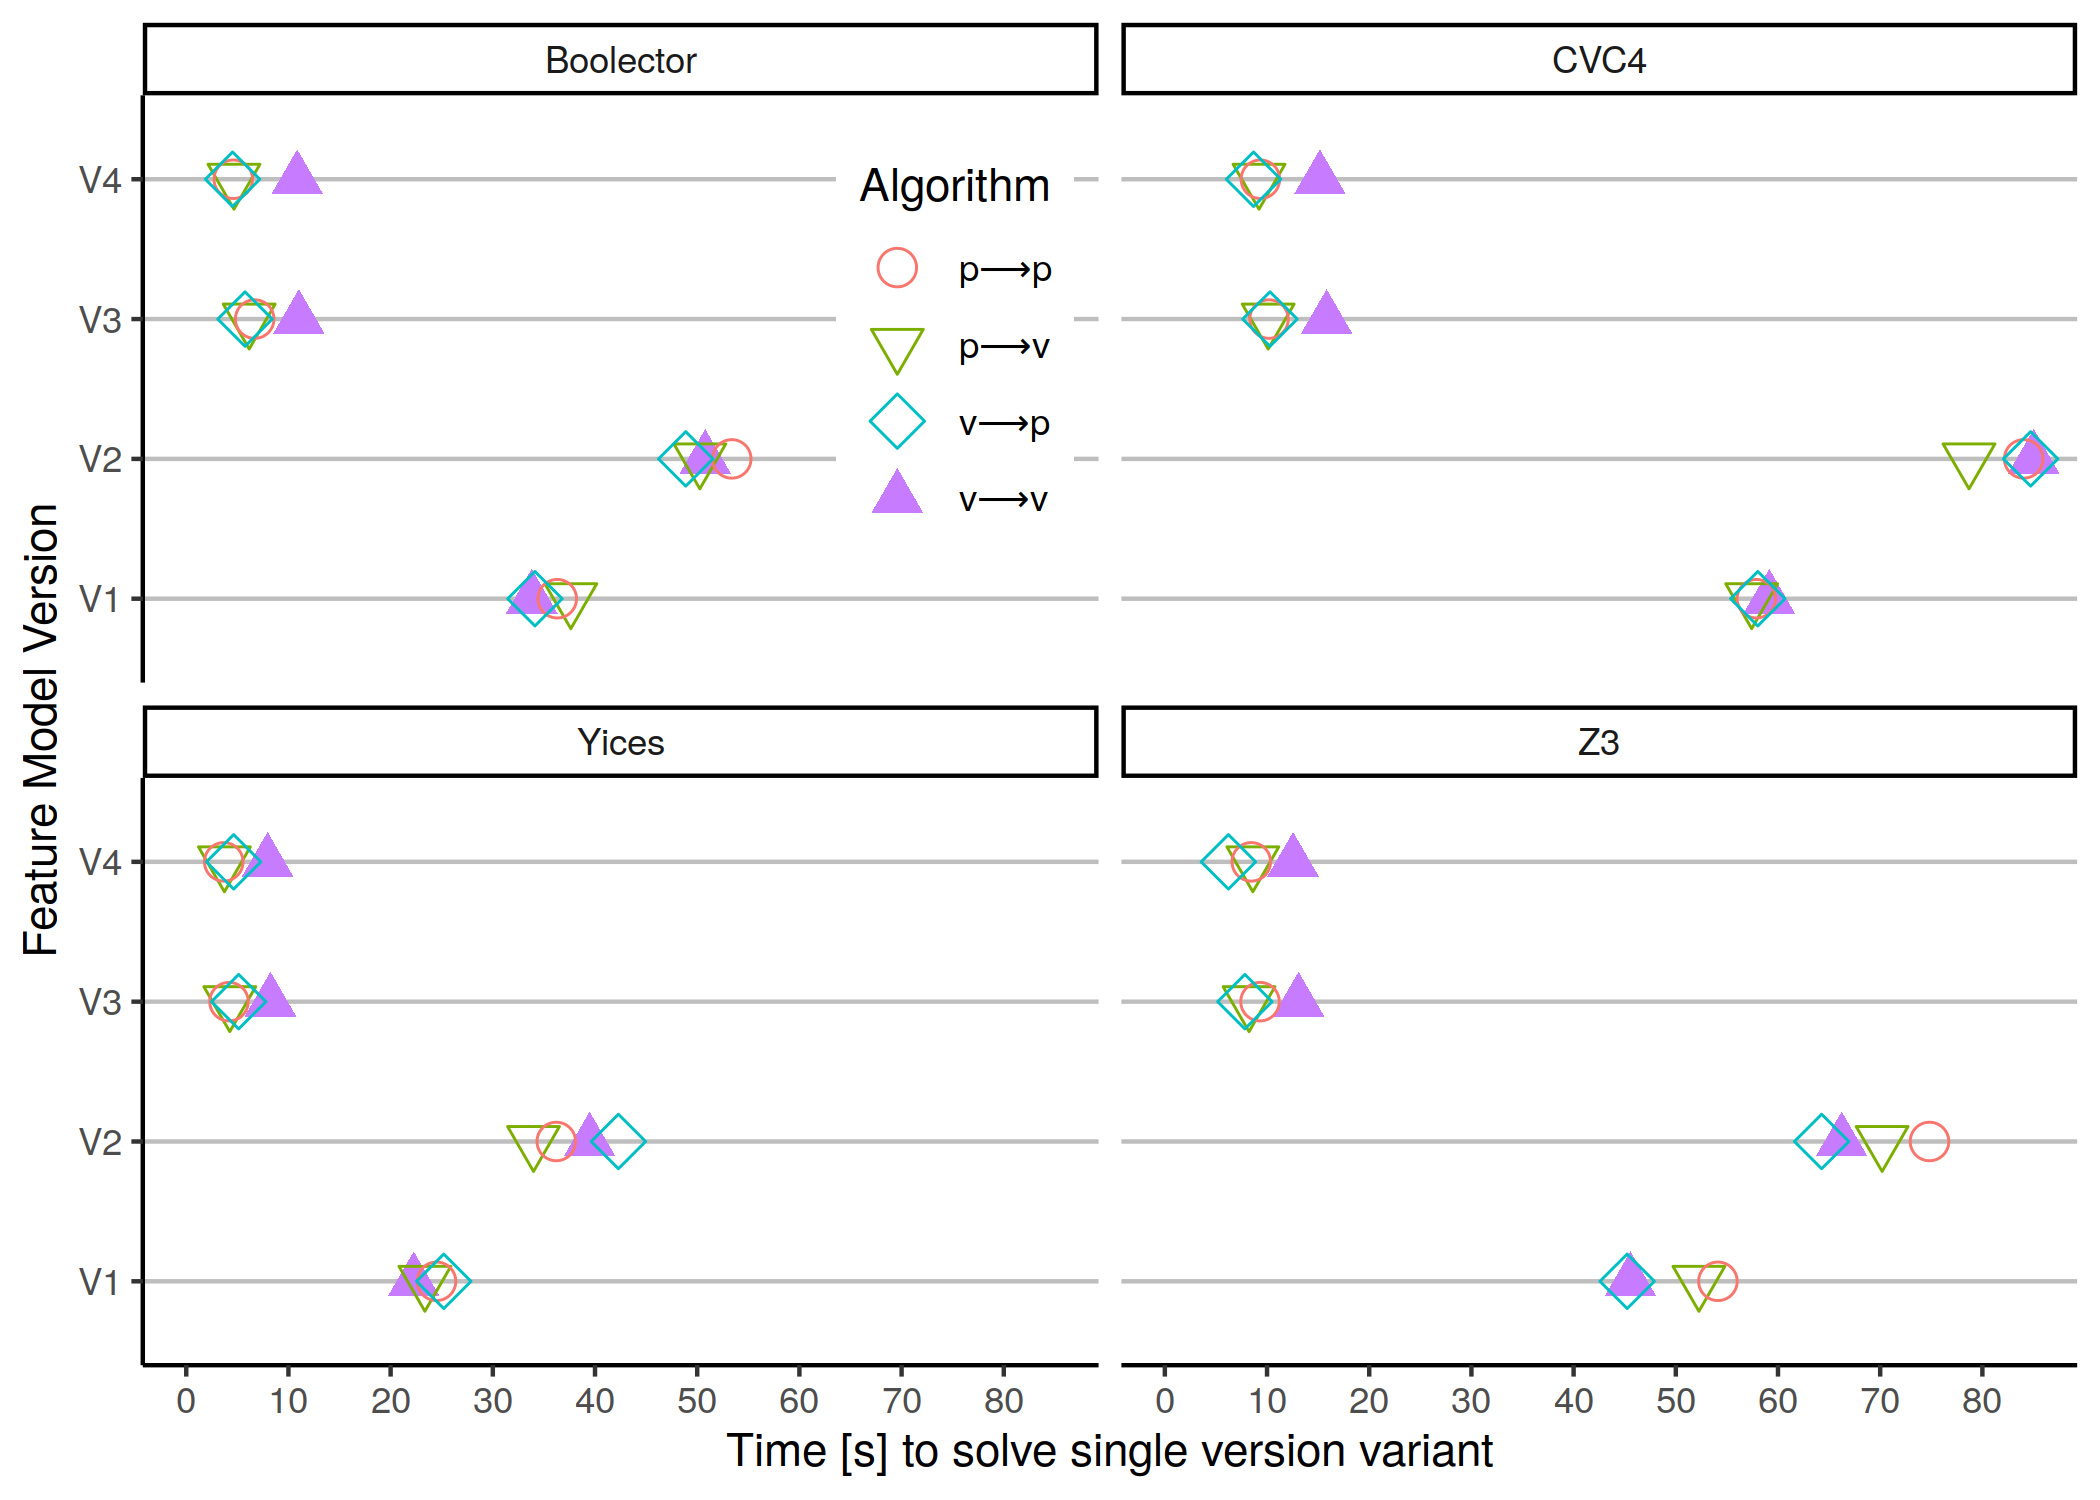
\includegraphics[width=0.95\textwidth]{Plots/RQ4_Auto}
    \caption{(Auto) RQ4: Overhead of \vTov{} on plain formulas. We observe that
      \vTov{} incurs an average slowdown of 9\% for \auto{}, when
      solving a version variant.}%
    \label{res:overhead:auto}
  \end{subfigure}
~
  \begin{subfigure}[t]{\textwidth}
    \centering
    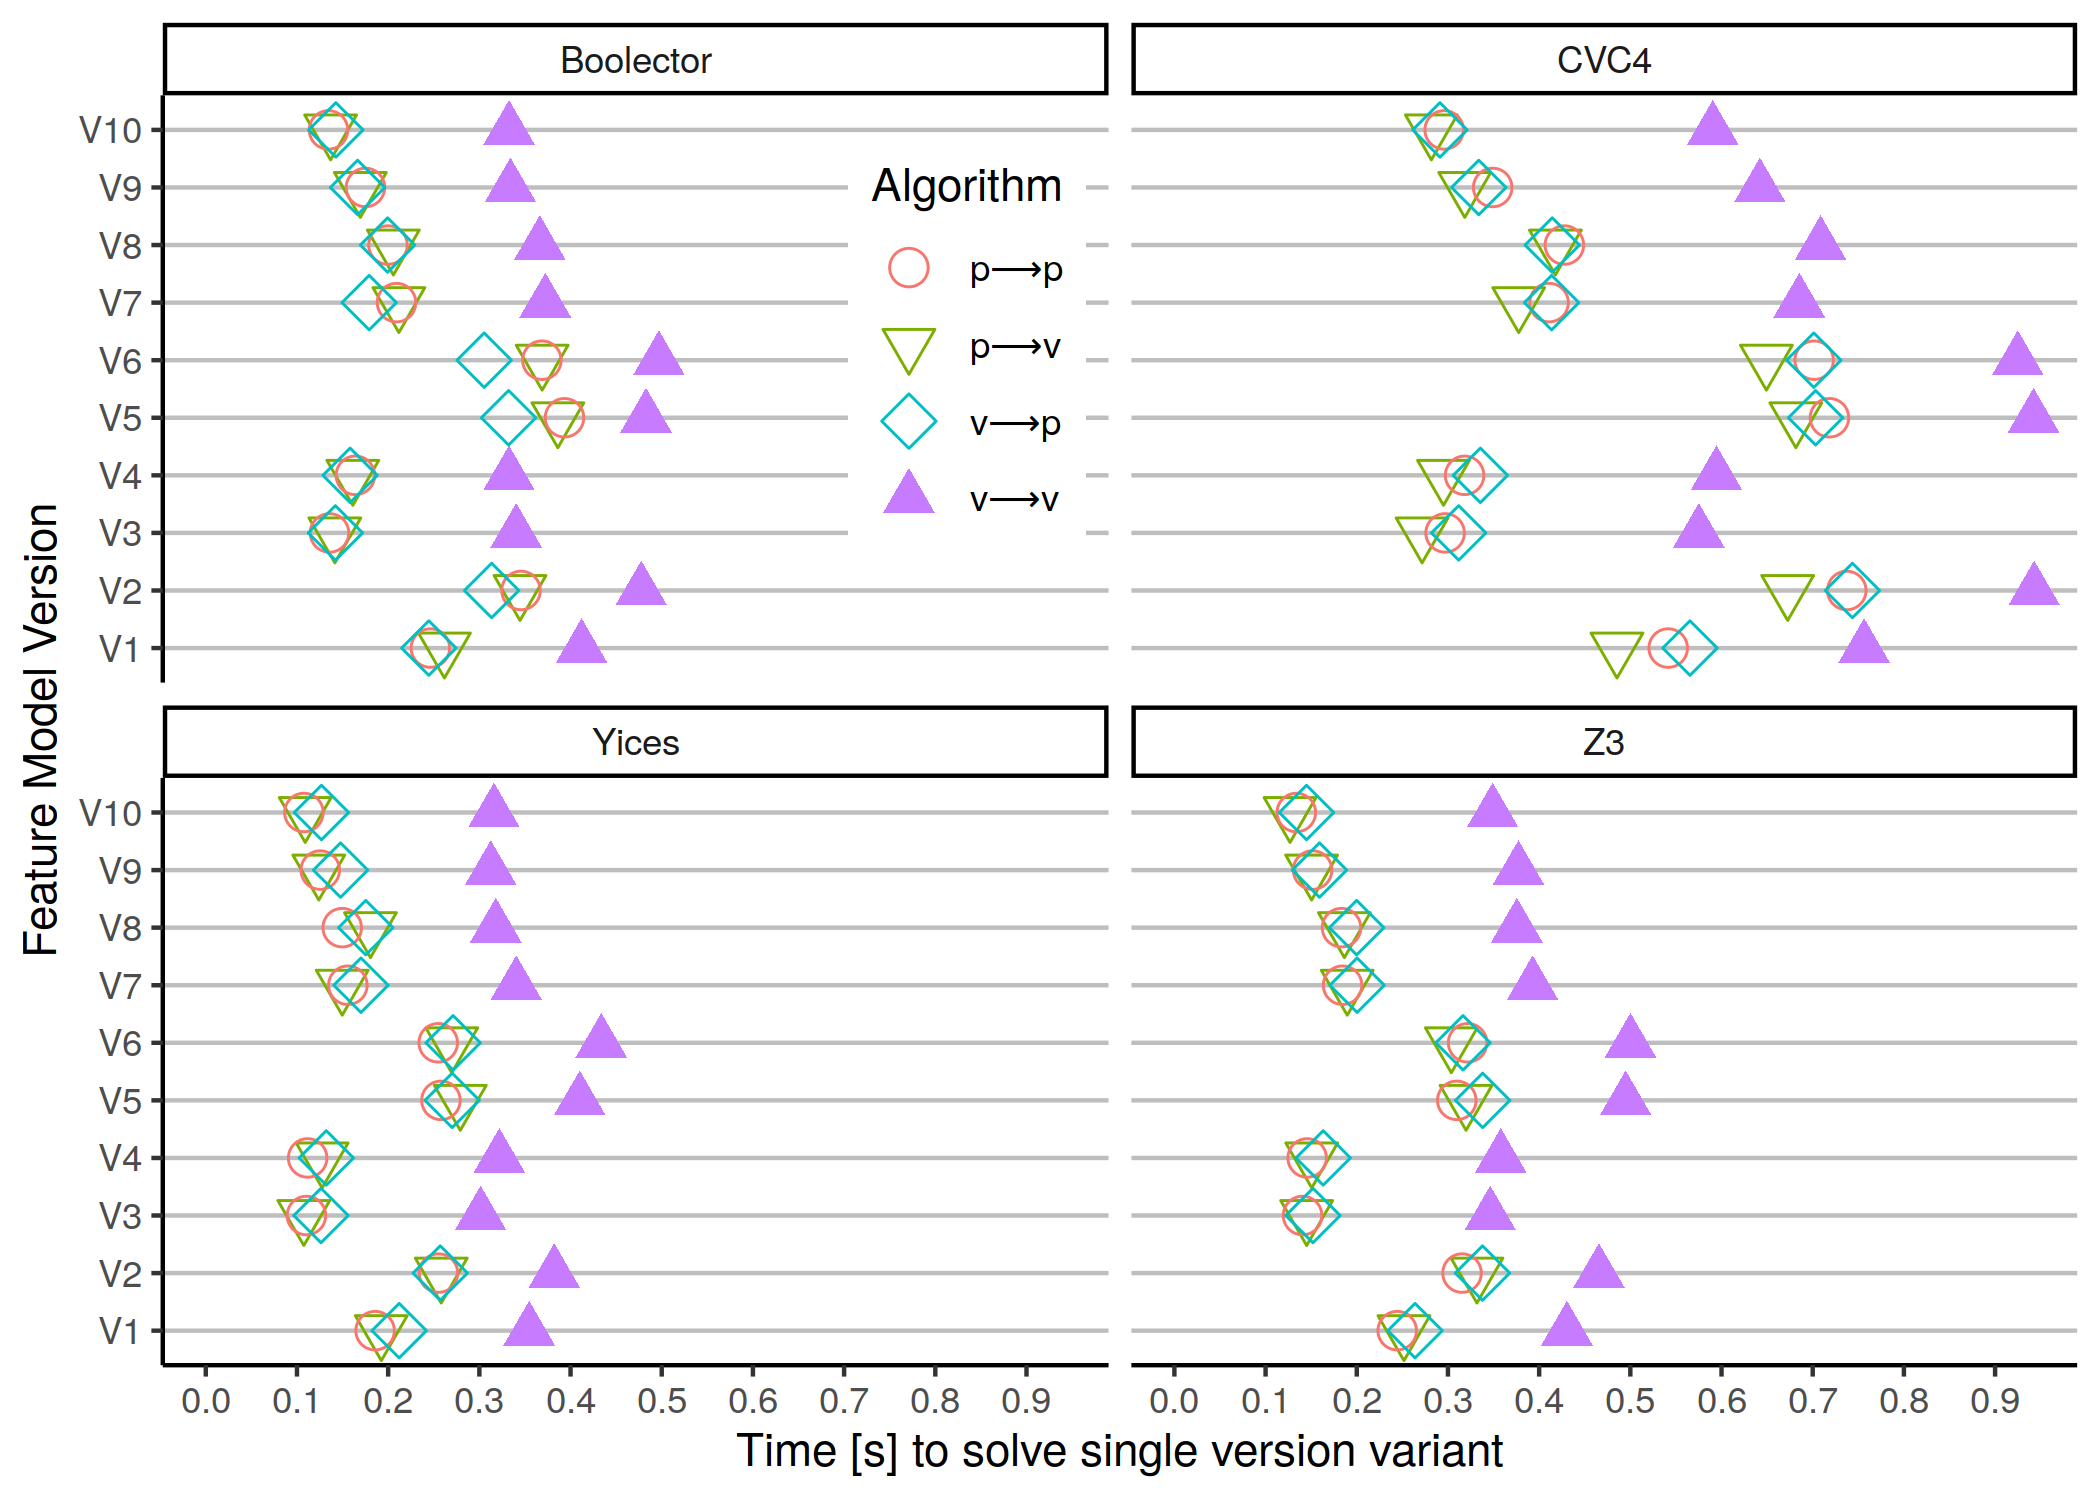
\includegraphics[width=0.95\textwidth]{Plots/RQ4_Fin}
    \caption{(Financial) RQ4: Overhead of \vTov{} on plain formulas. We observe
      that \vTov{} incurs an average slowdown of 75\% for the \fin{}
      dataset, when solving a version variant.}%
    \label{res:overhead:fin}
  \end{subfigure}
\end{figure}
%
\autoref{res:overhead:auto} and \autoref{res:overhead:fin} displays the
bootstrapped averages of each version variant, for each algorithm, and base
solver for the \auto{}, and \fin{} datasets, respectively. Given \resQ{2}, and
the composition of \fin{}, we expect \vsat{} to show slowdowns for \fin{}. This
is observed in \autoref{res:overhead:fin} and is statistically significant for
all versions. For \auto{}, only the $V_{1}$ version variant showed a significant
difference between the overhead case, \pTov{}, and \vTov{}, and between the
overhead case \pTov{}, and the typical case \vTop{}. Notably, \vTov{} did not
differ from the typical case, \vTop{}. \autoref{res:overhead:auto} suggests
statistically significant differences for other versions but omits variance,
hence the discrepancy between the plot and statistical tests. That \pTov{} was
statistically different for $V_{1}$ suggests particular formulas may not respond
well to the reduction engine, although the exact slowdown will be dependent on
the \ac{sat} problem.

\subsection{Threats to Validity}
Our results are subject to several threats to validity. Notably, we are unable
to make absolute performance claims because our study, with only two product
lines, may not be representative. To mitigate this we reused real-world data
from \nieke{}'s previous study~\citep{NMS+:GPCE18} and chose dissimilar product
lines. We inherit encoding-based threats to validity by reusing \nieke{}'s
formulas but ensured each algorithm experienced identical ordering of plain
terms as described in \autoref{section:case-studies:experimental-methodology}.
Furthermore our results, and our prototype solver are based on the widely used
Haskell library sbv. However, we believe this is a likely to be a common
implementation strategy for a variational solver (\ie{}, a solver built using a
library rather than a foreign function interface, similar to tools built on top
of sat4j~\citep{LP:JSAT10}) it is nonetheless a threat to validity as our
prototype directly depends on this library. To mitigate this threat we
maintained the same version of sbv throughout the experiment, employed it's
interface to interoperate for each base solver, and enforced the same code paths
through the library.

We have evinced the scalability claim with RQ1, and shown the translation and
automation of incremental solving in \autoref{chapter:vsat}. However, our
results depend on a \ac{vpl} formula as input and thus all points of variation
must be known before solving. We believe that \ac{vpl} formulas can be
incrementally and automatically constructed in practice, as new variants occur
or become known. However, assessing the challenges of \ac{vpl} construction is
left to future work, which we return to in
\autoref{section:conclusion:future-work}.

We do not provide a proof of the soundness of the prototype solver, although we
have showed variation preservation in
\autoref{section:vsat:variation-preservation}. We mitigate this threat in
several ways: we performed property-based testing~\cite{quickcheck} on our
prototype and verified that a satisfiable variant was found to be satisfiable
across all algorithms. In addition, we define a property that ensures that for
each plain model $p$, found with \pTov{}, \vTop{}, and \pTop{}, an satisfiable
model $p'$ was found by substituting $p$ on the variational model returned from
\vsat{}. We performed the property-based tests with 3,000 generated \ac{vpl}
formulas, finding no counter-examples.



%%% Local Variables:
%%% mode: latex
%%% TeX-master: "../../thesis"
%%% End:

\section{Variational \ac{smt} Results and Discussion}
~\label{section:case-studies:vsmt}
%
\begin{figure}
  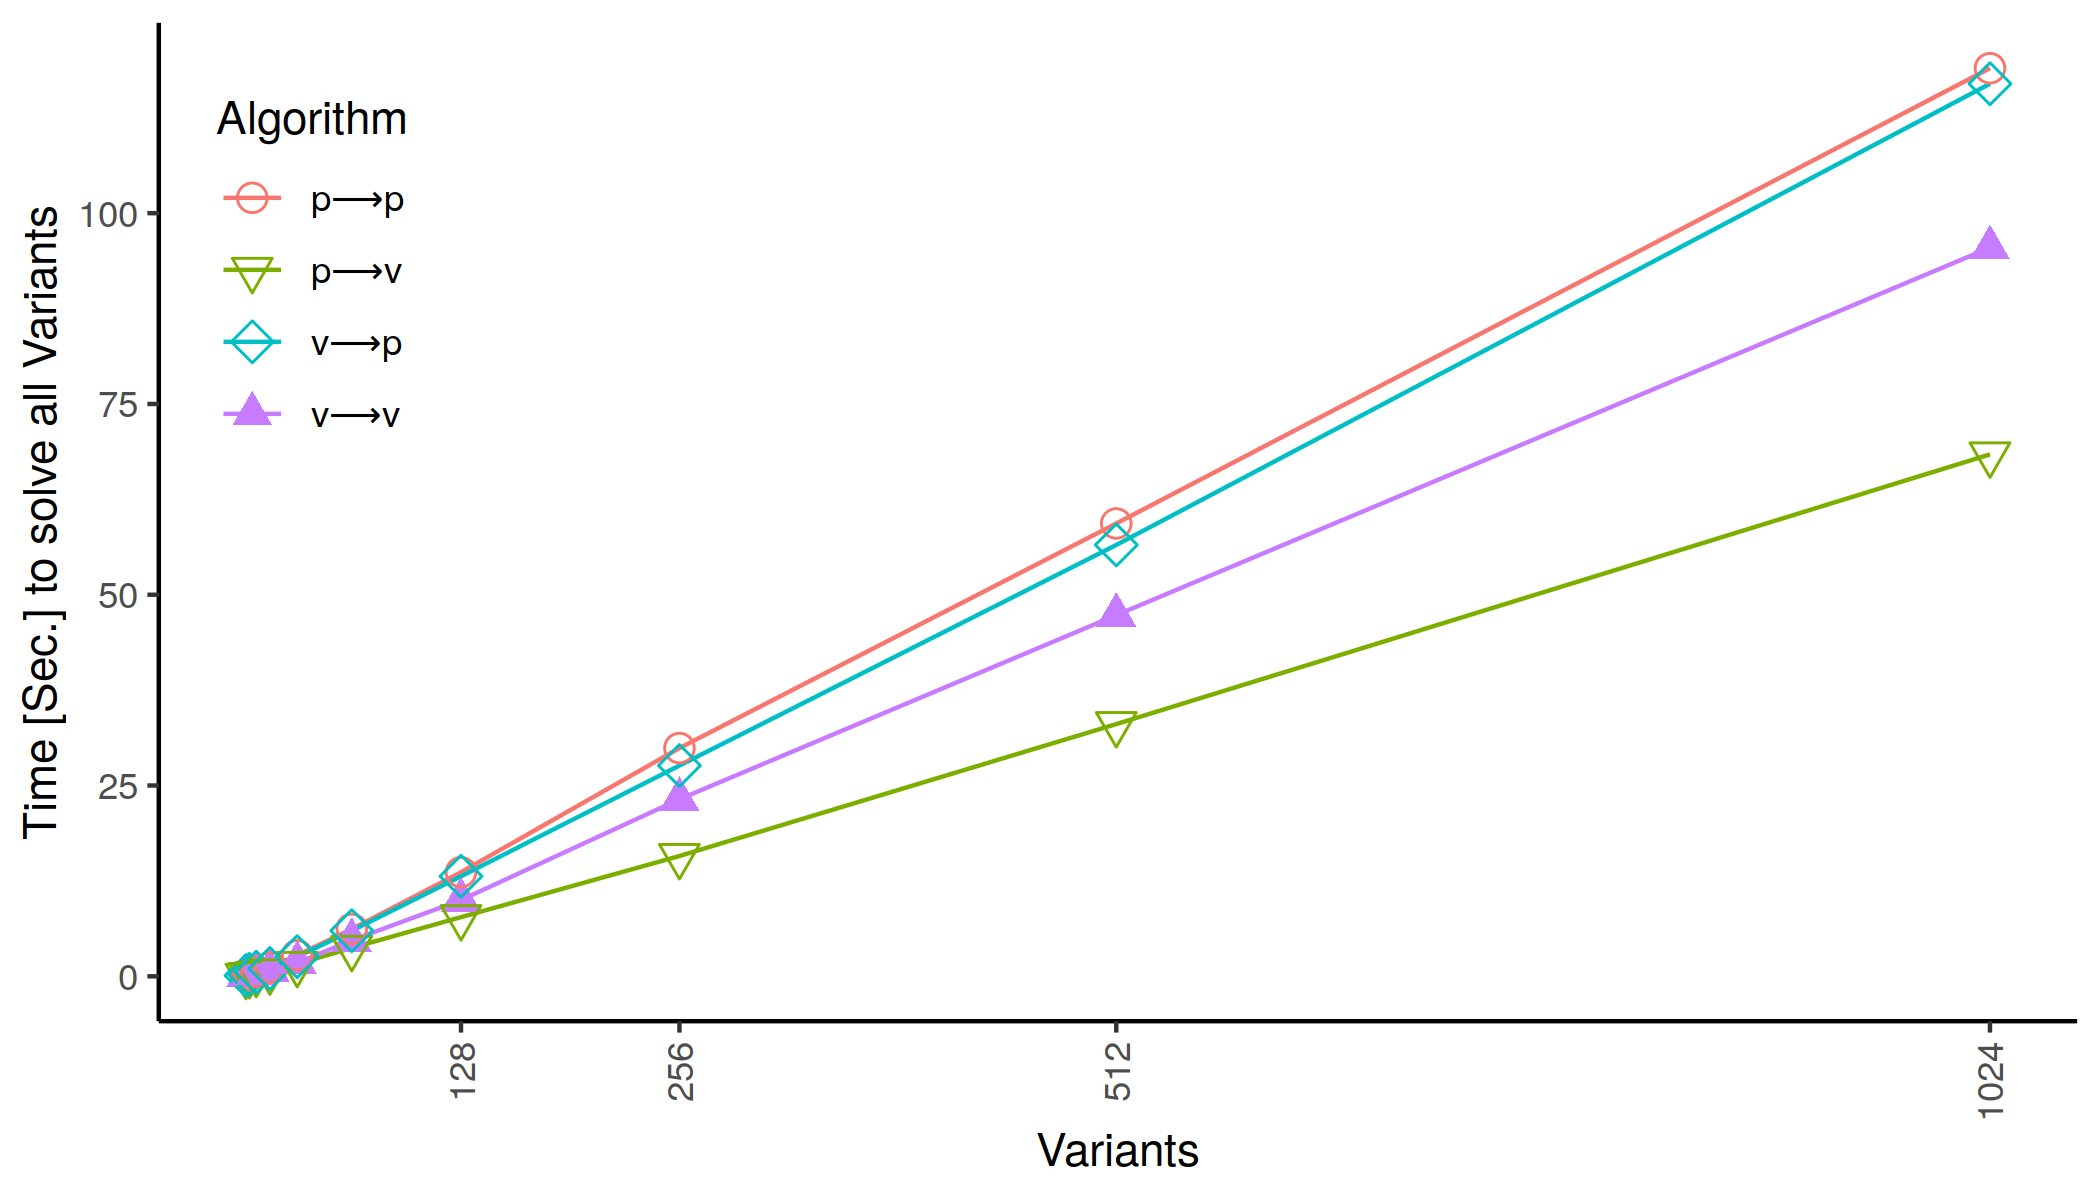
\includegraphics[width=0.95\textwidth]{Plots/RQ1_Fin_Smt}
  \caption{(Financial) Performance as variants increase for the variational
    \ac{smt} solver.}%
  \label{res:rq1:vsmt}
\end{figure}
%
We have shown that the variational \ac{sat} solver exhibits speedup for two
real-world datasets and that the sharing ration of a \ac{vpl} formula is a
significant factor in that speedup. However, we have yet to show that the same
is true for the prototype variational \ac{smt} solver, \vsmt{}.

To test \vsmt{} we use an \ac{smt} version of the \fin{} dataset from \nieke{}'s
study. Unfortunately, only the \fin{} dataset has an \ac{smt} version and so our
evaluation of the prototype \ac{smt} solver is limited. Furthermore, in the
course of encoding the dataset to a \evpl{} formula we discovered type errors
in 1,514 formulas out of a total of 4,621 formulas. To utilize the dataset we
detected and corrected the type errors during parsing. The type errors were
essentially identical and revolved around the encoding of a \rn{one-of}
constraint; where only one constraint out of a sequence of constraints can be
true. For example, an incorrect version would be: $(f_{i} \equiv{} 1) \equiv{}
(f_{0} + f_{1} \ldots{} + f_{n})$ for some $i$ and $n$. Thus, the error is that
$f_{i} \equiv 1$ yields a Boolean constraint (\ie{} $\equiv$ has type $\equiv{}
: \eAR{} \rightarrow \eAR{} \rightarrow{} \eIL{}$) but it is the left child of
another $\equiv$ which expects an arithmetic expression as its left child not a
\eIL{} expression. The correction is to repeat $f_{i}$ and handle the boolean
constraint correctly. For example the corrected version of the above formula is
$(f_{i} \equiv{} 1) \wedge{} (f_{i} \equiv{} (f_{0} + f_{1} \ldots{} + f_{n}))$,
where we separate out the left child from the summation but preserve the
semantics of the \rn{one-of} constraint.

\autoref{res:rq1:vsmt} displays the performance of \vsmt{} as variants to solve
increases. The resulting \evpl{} formula matched the number of choice and plain
terms from the \vsat{} version. Similarly, the number of satisfiable variants
matched the results for the \fin{} dataset in \autoref{res:vmodels}. \vsmt{}
displays a speedup of 1.22x over the baseline \vTop{} at 1,024 variants. There
are two significant differences between the \vsmt{} and \vsat{} results. First,
the prototype \ac{smt} solver \emph{does not} depend on the Haskell library
\texttt{sbv}. Instead, \vsmt{} utilizes a foreign-function interface to the C
API of z3. Consequently, where \texttt{sbv} utilizes strings over
\texttt{stdout} to communicate to the base solver, the ffi \vsmt{} uses utilizes
bytecode and hence has higher throughput. This has several implications, first,
the range of results \autoref{res:rq1:vsmt} are measured in seconds rather than
minutes such as \autoref{res:rq1:auto} and \autoref{res:rq1:fin}. Secondly, the
overhead case \pTov{} shows a speedup of 1.71x over the same baseline and is
consistently faster than the variational case \vTov{}. There are several
possible explanations while the exact reason is unclear. We speculate on
possible causes; the complete \pTov{} algorithm is given below:
%
\begin{lstlisting}[columns=flexible,keepspaces=true,language=Haskell]
  -- | Plain propositions on the variational solver testing the overhead of
  -- accumulate/evaluate
  pOnV :: [Plain Proposition] -> IO R.Result
  pOnV =  fmap mconcat . mapM (solve Nothing defSettings) . fmap unPlain
\end{lstlisting}

Which is in the form for a classic optimization technique in functional
programming called \emph{map fusion}\footnote{in practice fusion can lead to
  significant speedups ranging from 2x to an order of magnitude}\todo{cite map
  fusion and deforesting and average speedup} and thus could be highly optimized
by the Haskell compiler while the other algorithms where not. Furthermore,
\pTov{} computes the variant by accumulation/evaluation, reducing the entire
variant to a single symbolic and then issuing a \rn{check-sat} call. Thus, any
difference between \vTov{} and \pTov{} must come from choice removal.

This is significant because this result may be a case where the extra work
induced by the evaluation context for choice removal does not yield performance
increases. To be specific, \vTov{} constructs a context that to efficiently
reuse symbolic values, but if there exists a tautology or contradiction that is
plain, then \vTov{} will still construct and operate on this context even though
the result will be unchanged. Thus, it could be the case that for the majority
of variants a contradiction or tautology occurred and was found by z3 before the
local variation was considered (before the \rn{push}/\rn{pop} calls) and thus
any extra work to compute the result for the variant was redundant. The exact
reason for this result is unclear and more testing is required, however the
overall result: that \vTov{} still outperformed the baseline case \vTop{}, is
further demonstration of the success of our methods. Discovering the definitive
reason is left to future work. If an early tautology or contradiction is the
culprit then this could be addressed in an early optimization pass. Similarly,
if the Haskell compiler is optimizing \pTov{} and not optimizing the other
treatment conditions then this is an implementation detail which does not
invalidate our methods for variational \ac{sat} and \ac{smt} solving.

Lastly, the magnitude of difference in the runtime between the variational
\ac{smt} prototype and variational \ac{sat} difference is a significant result.
Such a difference is to be expected given their implementation differences, but
this difference indicates \emph{other} domains where applying variation as a
computational concept might be useful. As we have shown (perhaps unsurprisingly)
the performance benefits from using the concept of variation are greater when
the cost of a single transaction is high. For example, when the cost of emitting
a single string to the base solver is high, \eg{} in the prototype variational
\ac{sat} solver, we observe a greater performance speedup than we the cost is
low, \eg{} in the prototype variational \ac{smt} solver. Thus, it is likely that
other domains where a transaction cost is high are likely to benefit from
research on variation. These domains might include network communication, where
throughput and response times can be significant, or file systems and databases,
where disk accesses are the limiting performance factor. In either case, this
project successfully demonstrates performance speedups for two real-world cases
in \ac{sat} and \ac{smt} solving through the use of variational concepts.


%%% Local Variables:
%%% mode: latex
%%% TeX-master: "../../thesis"
%%% End: